% Dissertation presentation slides
% Zachariah Sharek

\documentclass{beamer}

\usepackage[english]{babel}
\usepackage[minionint,mathlf]{MinionPro}
\renewcommand{\sfdefault}{Myriad-LF}
\usepackage{graphicx}
\usepackage{xspace}
\usepackage{tabulary}

\newcommand{\deltap}{$\Delta P$}

% Fix colour shift problems
\pdfpageattr {/Group << /S /Transparency /I true /CS /DeviceRGB>>}

\renewcommand\sfdefault{phv}
\renewcommand\familydefault{\sfdefault}
\usetheme{default}
\usepackage{color}
\useoutertheme{default}
\usepackage{texnansi}
\usepackage{marvosym}
\definecolor{bottomcolour}{rgb}{0.32,0.3,0.38}
\definecolor{middlecolour}{rgb}{0.08,0.08,0.16}
\setbeamerfont{title}{size=\Huge}
\setbeamercolor{structure}{fg=gray}
\setbeamertemplate{frametitle}[default]%[center]
\setbeamercolor{normal text}{bg=black, fg=white}
\setbeamertemplate{background canvas}[vertical shading][bottom=bottomcolour, middle=middlecolour, top=black]
\setbeamertemplate{items}[circle]
\setbeamerfont{frametitle}{size=\huge}
\setbeamertemplate{navigation symbols}{} %no nav symbols

%\usetheme{Berlin}
%\setbeamertemplate{navigation symbols}{}
\useoutertheme{infolines} 

\author{Zachariah Sharek}
\title{The Illusion of the Illusion of Control}
\institute{Carnegie Mellon}
\date{May 3, 2012}

\begin{document}

\begin{frame}
	\titlepage
\end{frame}

\author{ }
\title{ }
\institute{ }
\date{ }


\section*{Outline}
\begin{frame}
	\tableofcontents
\end{frame}

\section{Control and Its Illusions}
\begin{frame}{Control}
	``A person's estimate that a given behavior will lead to certain outcomes.'' \\ 
	\textemdash Bandura, 1977\\
	\hyperlink{morecontroldefs}{\beamergotobutton{More definitions of control}}
\end{frame}

\begin{frame}{The Illusion of Control}
	``\textellipsis as an expectancy of a personal success probability inappropriately higher than the objective probability would warrant.'' \\
	\textemdash Langer, 1975
\end{frame}

\begin{frame}{My Question}
	Are people's estimates of control accurate?
	\pause
	Yes! But \textellipsis 
	\pause
	only if you ask them properly.
\end{frame}

\begin{frame}{Main Results of My Work}
	\begin{itemize}
	\pause
	\item People under-estimate control when it high
	\pause
	\item Perfectly normative information processors will also mis-estimate contingency
	\pause
	\item People are really good at estimating contingency in a Bayesian manner
	\pause
	\item People's view of control $\ne$ experimenters definition of control
	\pause
	\item Mis-estimates of control and accurate estimates of contingency occur in non-dichotomous cases
	\end{itemize}
\end{frame}

\subsection*{Preliminaries}
\begin{frame}{Our Universe of Discourse}
	\begin{figure}
	\begin{center}
		\includegraphics[width=\linewidth]{lightbulb}
	\end{center}
	\end{figure}
\end{frame}

\begin{frame}{Our Universe of Discourse}
	\begin{figure}
	\begin{center}
		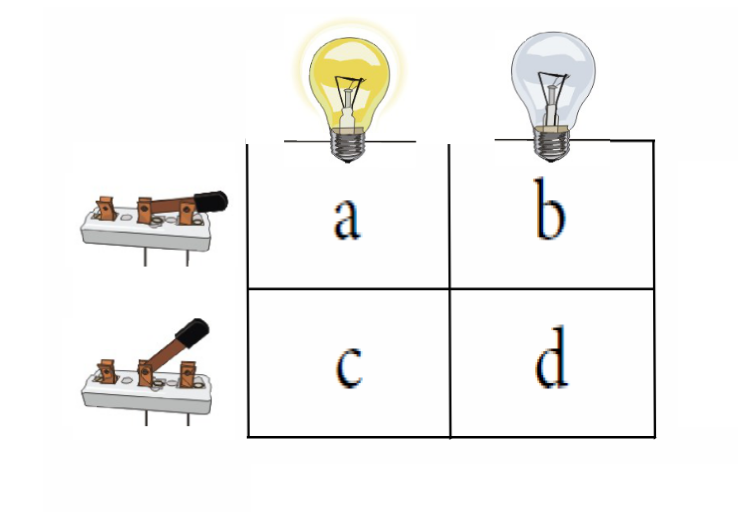
\includegraphics[width=\linewidth]{light_table}
	\end{center}
\end{figure}
\end{frame}

\begin{frame}{A Normative Measure of Control}
	\begin{figure}
	\begin{center}
		\includegraphics[width=\linewidth]{contingencytable}
	\end{center}
	\end{figure}
	$2 \times 2$ contingency matrix representing the joint frequencies of two binary input ($I$) and output ($O$) variables over $N$ trials, along with row and column sums.
\end{frame}

\begin{frame}{A Normative Measure of Control}
	\begin{figure}
	\begin{center}
		\includegraphics[width=\linewidth]{contingencytable}
	\end{center}
	\end{figure}
	\begin{equation*}
		\Delta P = P(O_1|I_1) - P(O_1|I_2) = a/(a+b) - c/(c+d)
	\end{equation*}
\end{frame}

\begin{frame}{A Normative Process for Control}
	\begin{enumerate}
		\item Find the \% of successes with one action: $P(O_1|I_1)$
		\item Find the \% of successes with the other action: $P(O_1|I_2)$
		\item Find the difference between these two numbers: \deltap
	\end{enumerate}
\end{frame}

\section{Keeping the Illusion of Control Under Control}
\begin{frame}{Keeping the Illusion of Control Under Control}
	Do people always over-estimate control?
	\pause
	\begin{figure}
	\begin{center}
		\includegraphics[width=\linewidth]{19880409}
	\end{center}
	\end{figure}
\end{frame}

\section{Modeling the Illusion of Control}
\subsection*{Bayesian Inference and the Illusion of Control}
	\begin{frame}{Bayesian Inference}
	\begin{equation*}
		p(H|D) = \frac{p(D|H)p(H)}{p(D)}
	\end{equation*}
		$p(H|D)$ is the posterior, the updated estimate of H\\
		$p(H)$ is the prior, the assumed hypothesis before data is observed\\ 
		$p(D|H)$ is called the likelihood and is the chance of data being observed if the hypothesis is true\\
\end{frame}

\begin{frame}{Bayesian Inference}
	\begin{equation*}
	f(\theta|Data) = \frac{f(Data|\theta)f(\theta)}{f(Data)} 
	\end{equation*}
	\pause
	\begin{displaymath}
	Posterior \propto Likelihood \times Prior
	\end{displaymath}
\end{frame}

\subsection*{Simulating the Illusion of Control}
\begin{frame}{Simulating the Illusion of Control}
	\begin{itemize}
		\item Imagine we run 1000 experiments
		\item Each experiment has $x$ subjects 
		\item Each subject is perfectly Bayesian
		\item Subjects press a button for $r$ rounds and observe the outcomes
		\item The button has a true probability of success, $\theta$
	\end{itemize}
\end{frame}

\begin{frame}{Simulating the Illusion of Control}
	\begin{itemize}
		\item The set of rounds per subject is a Binomial distribution:\\
	\begin{center}
		$f(Data|\theta) \sim Bin(r,\theta)$ 
	\end{center}
		\item The prior beliefs each subject has for $\theta$ can be modeled:\\
	\begin{center}
		$f(\theta) \sim Beta(\alpha,\beta)$ 
	\end{center}
		\item People's prior is usually $\sim$ 45\%
	\end{itemize}
\end{frame}

\begin{frame}{Simulation Results}
\begin{table} 	
	\setlength{\extrarowheight}{4pt}
	\begin{tabulary}{\linewidth}{LLL}
	\% Success & Empirical mean $\theta$  & Simulated mean $\theta$\\
	\hline
	90\% & 64.83\% & 65.19\%\\ 
	60\% & 47.00\% & 47.83\%\\
	\end{tabulary}
\end{table}
\end{frame}

\section{Study: Understanding Control}

\subsection*{Study Aims}
\begin{frame}{Understanding Control: Study Aims}
	\begin{itemize}
		\item Do people estimate control using \deltap \xspace as a normative model?
		\item How are estimates of the contingency between buttons and outcomes related to estimates of control?
		\item Do people process contingency information in a Bayesian manner?
	\end{itemize}
\end{frame}

\subsection*{Design}
\begin{frame}{Design}
	\begin{itemize}
		\item 165 participants paid \$1.25 on MTurk
		\item Two-button event-onset design
		\item One active button, ${\theta}_a$, one base-rate button, ${\theta}_b$
		\item Each round, must press a button and observe if it lights up a bulb.
		\item 100 total rounds---each button must be pressed 50 times
		\item Every 10 rounds per button, contingency, $p({\theta}_x)$, is elicited
	\end{itemize}
\end{frame}

\begin{frame}{Elicitation}
``We will ask you to estimate the likelihood that pushing Button A|B ten times in a row will produce 10 lit bulbs as well as estimating that pressing it ten times will result in 9,8,7,6,5,4,3,2,1 and 0 lit bulbs. These probabilities should reflect your own personal estimate of the number of times the light bulb would come on, given what you have observed.''
\end{frame}

\begin{frame}{Elicitation}
	\begin{figure}
	\begin{center}
		\includegraphics[width=\linewidth]{elicit_example_1}
	\end{center}
	\end{figure}
\end{frame}

\begin{frame}{Elicitation}
	\begin{figure}
	\begin{center}
		\includegraphics[width=\linewidth]{elicit_example_2}
	\end{center}
	\end{figure}
\end{frame}

\begin{frame}{Measures}
	\begin{itemize}
		\item Participants estimated the number of successes in 100 future trials for each button
		\item Incentivized for accuracy---bonus of \$0.50
		\item Asked for personal definition of control
		\item Then use that definition to estimate their control on scale (0--100)
	\end{itemize}
\end{frame}

\subsection*{Results}

\begin{frame}{Results: Control Estimates}
	\begin{table} 	
		\setlength{\extrarowheight}{4pt}
		\begin{tabulary}{\linewidth}{rLLLL}
		\hline
		Condition & Active \% & Base \% & Control ($\Delta P$) & Mean Estimated Control (SD)\\
		\hline
		1 & 100\% & 50\% & 50\% & 42.34\%  (35.93)\\ 
		2 & 50\%  & 50\% & 0\%  & 24.64\%* (26.13)\\
		3 & 100\% & 20\% & 80\% & \mbox{40.25\%* (25.76)}\\
		4 & 20\%  & 20\% & 0\%  & 19.21\%* (22.96)\\
		5 & 70\%  & 20\% & 50\% & 26.97\%* (27.68)\\
		\hline	 	
		\end{tabulary}	
	\end{table}
\end{frame}

\begin{frame}{Results: Contingency Estimates}
	\begin{table} 	
		\setlength{\extrarowheight}{4pt}
		\begin{tabulary}{\linewidth}{rlll}
		\hline
		Condition & Control ($\Delta P$) & Est. Control & Est. Contingency\\
		\hline
		1 & 50\% & 42.34\%  (35.93) & 44.91\% (14.9)\\ 
		2 & 0\%  & 24.64\%* (26.13) & 4.18\% (12.0)\\
		3 & 80\% & 40.25\%* (25.76) & 59.86\%* (27.3)\\
		4 & 0\%  & 19.21\%* (22.96) & 1.2\% (11.4)\\
		5 & 50\% & 26.97\%* (27.68) & 41.48\%* (20.4)\\
		\hline	 	
		\end{tabulary}	
	\end{table}
\end{frame}

\begin{frame}{Contingency to Control}
	Estimates of contingency and control are not correlated!*
	\begin{figure}
		\begin{center}
			\includegraphics[width=\linewidth]{control_contingency}
		\end{center}
	\end{figure}
\end{frame}

\begin{frame}{Sympathy for Participants}
\begin{itemize}
\item We can compare estimates of contingency to observations
\item Run a binomial test on each participant
\item Non-significant results = \emph{reasonable}
\item Out of 165, 110 (66\%) were reasonable for both buttons
\item Most people are quite accurate!
\end{itemize}
\end{frame}

\begin{frame}{How Bayesian were participants?}
	\begin{table}
	\begin{tabulary}{\linewidth}{CCCCCCC}
	\hline
	 & \multicolumn{3}{c}{Button A Modal \%} & \multicolumn{3}{c}{Button B Modal \%} \\ 
	 &  Est. & Bayes & Act. & Est.  & Bayes & Act. \\ 
	\hline
	1 & 85   & 100  & 100 & 47.2 & 51.56 & 50 \\ 
	2 & 43.1 & 46.9 & 50  & 48.7 & 48.0  & 50 \\ 
	3 & 86.9 & 100  & 100 & 21.4 & 21.7  & 20 \\ 
	4 & 17.9 & 18.6 & 20  & 22.4 & 17.6  & 20 \\ 
	5 & 57.9 & 71.0 & 71  & 24.1 & 20.3  & 20 \\ 
	\hline
	\end{tabulary} 	
	\end{table}
\end{frame}

\begin{frame}{Button A: Participants vs. Bayesians}
	\begin{figure}
	\begin{center}
		\includegraphics[width=\linewidth]{bayesian_bar_button_A}
	\end{center}
	\end{figure}
\end{frame}

\begin{frame}{Button B: Participants vs. Bayesians}
	\begin{figure}
	\begin{center}
		\includegraphics[width=\linewidth]{bayesian_bar_button_B}
	\end{center}
	\end{figure}
\end{frame}

\begin{frame}{Bayesian comparison}
	\begin{figure}
	\begin{center}
		\includegraphics[width=\linewidth]{learning1}
	\end{center}
	\end{figure}
\end{frame}


\begin{frame}{Bayesian comparison}
	\begin{figure}
	\begin{center}
		\includegraphics[width=\linewidth]{learning2}
	\end{center}
	\end{figure}
\end{frame}


\begin{frame}{Bayesian comparison}
	\begin{figure}
	\begin{center}
		\includegraphics[width=\linewidth]{learning3}
	\end{center}
	\end{figure}
\end{frame}


\begin{frame}{Bayesian comparison}
	\begin{figure}
	\begin{center}
		\includegraphics[width=\linewidth]{learning4}
	\end{center}
	\end{figure}
\end{frame}


\begin{frame}{Bayesian comparison}
	\begin{figure}
	\begin{center}
		\includegraphics[width=\linewidth]{learning5}
	\end{center}
	\end{figure}
\end{frame}

\begin{frame}{Study Conclusions}
\begin{itemize}
	\item Similar patterns of control estimates to previous studies
	\item Estimates of contingency are generally accurate
	\item Estimates of control are not correlated to estimates of contingency
	\item Estimates of contingency are processed in a Bayesian-like manner
\end{itemize}
\end{frame}

\section{Study: Understanding Control Redux}
\subsection*{Study Aims}
\begin{frame}{Understanding Control Redux: Study Aims}
	\begin{itemize}
		\item Perhaps results in previous study were due to the forced sampling and elicitation?
		\item Relaxing these requirements should lead to:
		\begin{enumerate}
		\item Less sampling, leading to more regressive estimates
		\item Less elicitation leading to less accurate contingency estimates
		\end{enumerate}
		\item How would people respond to \deltap?
	\end{itemize}
\end{frame}

\subsection*{Design}
\begin{frame}{Design}
	\begin{itemize}
		\item Similar to the previous study---two button event-onset
		\item 138 participants through MTurk, paid \$0.75 and incentive of \$0.50 for accuracy
		\item No Bayesian elicitation and subjects could sample as much (or little) as desired	
	\end{itemize}
\end{frame}

\subsection*{Results}
\begin{frame}{Results}
	\begin{table} 	
		\setlength{\extrarowheight}{4pt}
		\begin{tabulary}{\linewidth}{LLLLL}
		\hline
		Actual Control & BIOC Control & BIOC \deltap & \mbox{Control} & Est. \deltap\\
		\hline
		50\% & 42.34\%  & 44.91\%  & 63.6\%* & 48.8\%\\ 
		0\%  & 24.64\%* & 4.18\%   & 34.7\%* & 2.2\%\\
		80\% & 40.25\%* & 59.86\%* & 68.4\%  & 84.1\% \\
		0\%  & 19.21\%* & 1.2\%    & 17.3\%* & 1.2\%\\
		50\% & 26.97\%* & 41.48\%* & 28.3\%* & 45.6\%\\
		\hline	 	
		\end{tabulary}	
	\end{table}
\end{frame}

\begin{frame}{Introducing \deltap}
One way to measure the amount of control that people have in this situation with the light bulbs is to measure the percentage of times the light bulb comes on when you press Button A and when you press Button B. The difference between these two percentages is the amount of control your choice of which button to press has on the light bulb. 

For example, from your answers, you would expect Button A to light the light bulb up X\% of the time and Button B to work Y\% of the time. Thus, according to this measure of control, you would expect to have $(X - Y)\%$ control over making the light bulb light up. 

Do you agree with this definition of control? 
Please use the following scale below to indicate how strongly you agree with this suggested definition of control. (1--7 scale)
\end{frame}

\begin{frame}{Responses to \deltap}
Scale from 1=Strongly Disagree, 4=Neither Agree nor Disagree, 7=Strongly Agree
	\begin{table}
		\centering 	
		\begin{tabulary}{\linewidth}{rLL}
		\hline
		Condition & Mean Agreement     & \% Favoring \\
		          & with \deltap \xspace (SD)  & \deltap \xspace (N)    \\
		\hline
		1 & 4.5 (2.0) & 17.9\% (5) \\ 
		2 & 4.9 (1.3) & 19.4\% (7) \\
		3 & 4.4 (2.2) & 18.1\% (4) \\
		4 & 5.3 (1.4) & 42.3\% (11)\\
		5 & 3.9 (1.8) & 26.0\% (6) \\	
		\hline
		\end{tabulary}
	\end{table}
\end{frame}

\begin{frame}{Conclusion}
	\begin{itemize}
		\item People did sample less: M=66.5 (SD=68.5)
		\item \deltap \xspace is not embraced as a normative measure by participants
		\item People were still quite accurate, but not regressive
		\item Lack of a formal elicitation mechanism did not appear to affect accuracy
	\end{itemize}
\end{frame}

\section{Study: Non-Dichotomous Control}
\begin{frame}{Study: Non-Dichotomous Control}
	\begin{itemize}
		\item Many of the outcomes of our efforts are not on/off
		\pause
		\item Stocks
		\pause
		\item Manufacturing output
		\pause
		\item Performance measures
	\end{itemize}
\end{frame}

\subsection*{Extending \deltap}
\begin{frame}{Extending \deltap}
	\begin{equation*}
		\Delta P = P(O_1|I_1) - P(O_1|I_2)
	\end{equation*}
	\begin{itemize}
		\item How can we adapt \deltap \xspace for non-dichotomous situations?
		\item $O_1$ represents success
		\item We need to define a new threshold of success
	\end{itemize}
\end{frame}

\begin{frame}{Extending \deltap}
	\begin{equation*}
		\Delta P = P(O_1|I_1) - P(O_1|I_2)
	\end{equation*}
	\begin{itemize}
		\item Imagine we are evaluating two widget producing machines, A and B.
		\item $I_1$ is machine A, $I_2$ is machine B
		\item $O$ is the number of widgets produced
		\item Define success as 100 or more widgets produced
	\end{itemize}
\end{frame}

\begin{frame}{Extending \deltap}
	\begin{displaymath}
	\Delta P = P(O \ge 100|A) - P(O \ge 100|B)
	\end{displaymath}
	\begin{itemize}
		\item Imagine we are evaluating two widget producing machines, A and B.
		\item $I_1$ is machine A, $I_2$ is machine B
		\item $O$ is the number of widgets produced
		\item Define success as 100 or more widgets produced
	\end{itemize}
\end{frame}

\begin{frame}{Extending \deltap}
	\begin{displaymath}
	Extended \Delta P = P(O \ge 100|A) - P(O \ge 100|B)
	\end{displaymath}
	\begin{itemize}
		\item If A and B have the exact same probability distribution then \deltap \xspace is 0
		\item Suppose they have different parameters or different families?
		\item How can we calculate this?
	\end{itemize}
\end{frame}
	

\begin{frame}{Extending \deltap}
	\begin{displaymath}
	Extended \Delta P = -F_A(x) - F_B(x) \; \mbox{where} \; F_X(x) = P(X \le x) 
	\end{displaymath}
	\pause
	\begin{displaymath}
	Extended \Delta P = -F_A(100) - F_B(100) \; \mbox{where} \; F_X(100) = P(X \le 100) 
	\end{displaymath}		
\end{frame}	

\subsection*{Study Aims}
\begin{frame}{Study Aims}
	\begin{itemize}
		\item Is this extension an accurate measure of control?
		\item Demonstrate that people will show the same pattern of control estimates as previous studies
	\end{itemize}
\end{frame}

\subsection*{Design}
\begin{frame}{Design}
	\begin{itemize}
		\item 99 participants recruited on MTurk and paid \$1.00
		\item Assume the role of a factory manager testing two widget-making machines
		\item Each machine needs to be tested 50 times
	\end{itemize}
\end{frame}

\begin{frame}{Measures}
	\begin{itemize}
		\item Estimate the average number of widgets produced by each machine in 100 runs
		\item ``How much control of widget production did your choice of Machine A vs. B give you?''
		\item ``If your goal was to produce 600 or more widgets, how much control did your choice of Machine A vs. B give you in achieving your goal?''
	\end{itemize}
\end{frame}

\begin{frame}{Conditions}
	\begin{table}
		\centering 	
		\begin{tabulary}{\linewidth}{rLLL}
		\hline
		Condition & Machine A Mean (SD) & Machine B Mean (SD) & Control $(X \ge 600)$\\
		\hline
		1 & 500 (100) & 500 (100) & 0\%\\ 
		2 & 700 (100) & 500 (100) & 68.3\%\\
		\hline
		\end{tabulary}
	\end{table}
\end{frame}

\subsection*{Results}
\begin{frame}{Results: Estimates of Control}
	\begin{table}
		\centering 	
		\begin{tabulary}{\linewidth}{LLLL}
		\hline
		Machine A Est. Mean (SD) & Machine B Est. Mean (SD) & Est. Control & Est. Control $(X \ge 600)$\\
		\hline
		511.6 (96.14) & 497.5 (79.19) & 23.9\% (27.8) & 33.67\%* (30.78)\\ 
		671.9 (107.9) & 475.9 (86.33) & 39.0\% (32.8) & 61.0\% (30.78)\\
		\hline
		\end{tabulary}
	\end{table}
\end{frame}

\begin{frame}{Results: Estimates of Means}
	\begin{itemize}
		\item If we compare the difference in means:
		\item (Machine A estimate - Machine B estimate) - (Machine A actual mean - Machine B actual mean) = 0
		\item This comparison is not significantly different from 0 (M=2.22, SD=69.7)	
	\end{itemize}
\end{frame}

\begin{frame}{Non-dichotomous Conclusion}
	\begin{itemize}
		\item Participants' estimates of outcomes are accurate
		\item Estimates of control are not accurate---Different definition of control?
		\item Does extended \deltap \xspace work?
	\end{itemize}
\end{frame}


\section{Conclusion}

\subsection*{Causes of Control?}
\begin{frame}{Causes of Control?}
	\begin{itemize}	
		\item Thompson et al. (1998) suggested the control heuristic
		\item Estimates of control are affected by perceptions of:
			\begin{itemize}
				\item Intentionality
				\item Connection
			\end{itemize}
		\item This doesn't explain the uncoupling of contingency and control	
	\end{itemize}
\end{frame}

\begin{frame}{Attribute Substitution?}
	\begin{itemize}	
		\item Perhaps people are answering a different question when their estimate of control is elicited?
		\item Kahneman \& Frederick (2002) propose a new explanation for the representativeness heuristic
		\item When asked a question, people \emph{substitute} difficult attributes with easier attributes
		\item ``How much control did your choice of button A or button B have on the light bulb lighting up?''
		\pause
		\item ``How much success did you have in making the light bulb light up?''
	\end{itemize}
\end{frame}

\subsection*{Implications}
\begin{frame}{Implications \& Future Research}
	\begin{itemize}	
		\item Taylor \& Brown (1988) argue that positive illusions are adaptive
		\item Base their argument on ``depressive realism'' (e.g. Abramson \& Alloy, 1981)
		\item Dykman et al. (1989) show that depressed estimates are in fact, just depressed
		\item Perhaps the adaptive benefits of the illusion of control are due to possessing a belief of at least some control?
	\end{itemize}
\end{frame}

\begin{frame}{Implications \& Future Research}
	\begin{itemize}	
		\item Overconfidence shows a similar pattern of results to control estimation
		\item Emerson's definition of power = \deltap
		\item Correspondence bias: perhaps people partition judgements into controllable and not controllable?
	\end{itemize}
\end{frame}

\begin{frame}{Implications \& Future Research}
	\begin{itemize}	
		\item More (statistical) work on what factors affect estimates of control
		\item Better understanding of people's definitions of control
		\item More realistic experiments
		\begin{itemize}
			\item Control in ethical decision-making
		\end{itemize}
	\end{itemize}
\end{frame}

\subsection*{Summation}
\begin{frame}{Main Results of My Work}
	\begin{itemize}
	\item People under-estimate control when it high
	\item Perfectly normative information processors will also mis-estimate contingency
	\item People are really good at estimating contingency in a Bayesian manner
	\item People's view of control $\ne$ experimenters definition of control
	\item Mis-estimates of control and accurate estimates of contingency occur in non-dichotomous cases
	\end{itemize}
\end{frame}
\begin{frame}{Summation}
	\begin{itemize}
	\item These results indicate that people do not consistently over-estimate their control
	\item If we ask them nicely, they give us the ``correct'' answers
	\item Thus, my evidence suggests that the illusion of control is an illusion
	\end{itemize}
\end{frame}

\subsection*{}
\begin{frame}
Thank You!
\end{frame}


\appendix

\section{Definitions of Control}
\begin{frame}[label=morecontroldefs]{More Definitions of Control}
\begin{itemize}
\item ``The concept of control may be defined in terms of perceptions of contingencies.  If a person perceives a contingency between his behaviors and an outcome \textellipsis outcome is considered controllable.''  \textemdash Glass and Carver, 1980
\item ``The accumulation of action-outcome episodes that accrue based on an individual's actions in a set of objective control conditions which are interpreted according to his or her subjective control beliefs.'' \textemdash Skinner, 1985
\item Base Rate: ``The subjective probability with which the current situation will lead to a future outcome without action'' \textemdash Heckhausen, 1977
\item Actual control: ``The measure of actual control that subjects are given is directly tied to the amount of change the environment allows the subjects to effect'' \textemdash Chanowitz and Langer, 1980
\end{itemize}
\end{frame}

\begin{frame}
The End!
\end{frame}

\end{document}